\chapter{\label{sec:implementation}Implementation}

% - module discovery gossip
% - rating and voting
% - code screenshots
% - LoC + code coverage stats

This chapter discusses the design principles and implementation details of the system described in the previous chapter. This work took a prototyping approach to get to a functioning prototype rapidly and improve from there. The sections below we explain the different functionalities that were tackled in chronological order.

\section{Module Distribution}

The first step that was taken to undertake this project was module distribution. Distribution was chosen as the idea hinges on the ability to setup an integrated content distribution network that would work efficiently and scale. Since this is not the first time this is done and there already exist excellent solutions out there that could accomplish this. Below I will list the different protocols considered.

\subsection{Protocols}
\subsubsection{\textbf{TFTP}}
Trivial File Transfer Protocol (TFTP) is a very simple and old file transfer protocol. It is mostly used in older enterprise equipment and is not really used anymore today. This has to due with the downsizes of the protocol in that it has no security built-in and has no verification that the content has arrived intact.

\subsubsection{\textbf{FTP(S)}}
File Transfer Protocol is a newer protocol than TFTP, but still older than the other alternatives. This protocol is mostly used for transferring content to web servers. For that purpose this protocol functions well because it is lightweight, provides content verification, and is simple. The downside for our use-case is that it isn't secure by default (gets routed through a HTTPS connection), doesn't support file transfer resumes, and doesn't scale well.

\subsubsection{\textbf{Web protocols}}

Web protocols like HyperText Transfer Protocol (HTTP) and its secure variant HTTPS are a very common transfer protocol in the current day internet. It is used by all major Linux distribution to distribute the system packages, by websites for downloading content and watching videos. This protocol supports file transfer resumes, encryption. It, However, doesn't scale well when the same content has to be uploaded to multiple users and doesn't natively provide content verification.

\subsubsection{\textbf{BitTorrent}}

BitTorrent is the protocol used by all bittorrent clients. It provides encryption, content verification, file transfer resumes, and scales very well when large amounts of the same contents has to be distributed thanks to its mesh architecture. That is why this protocol was selected as the basis of the module distribution of this work.

\subsection{Module transfer protocol}
Several small experiments were conducted to test the feasibility of the BitTorrent protocol with the regards to this work its use-case. These were related to choosing a suitable BitTorrent implementation, testing the creation of a torrent and downloading this just created torrent on multiple other nodes. We made use of magnet links to transfer the information required to download the torrent. Ones these experiments were deemed successful, we had to find a way to distribute this magnet link through the network without using the traditional method of content indexing services. The method that we chose is described in the discovery section.

\section{Discovery and Voting protocol}

When a suitable transfer protocol is chosen, the next step was to make it possible for modules to be discoverable by all nodes in the system. Since we were already building our framework on top of the IPv8 peer-to-peer communication library. We decided it would be a good fit to use this to accomplish our goal, since it was very suited for bulk small size data gossiping. So this became out chosen method of module discovery.

Since IPv8 also provides a block-chain storage back-end it was an perfect opportunity to 

\section{Module Design}

\section{Event-Driven Architecture}

\section{GUI integration}

\section{Code review}

\chapter{Mobile App}

To test the robustness and the flexibility of the framework, an experiment was performed to try to create a proof-of-concept prototype of an Android application that could run the same stack of code to extend the ecosystem to mobile platforms. Since the two major mobile platforms (Android, iOS) only run applications custom made for these platforms, different methods had to be explored. Because iOS has a very restricted development environment and strict security policies, this route was not further explored.

The Android platforms allows app developers to run Java, Kotlin (Java based), and C. The desired framework language (Python) does not natively run on this platform. Converting the project code and dependencies is not a simple or maintainable method. This approach, however, also would not work. To improve security, the Android platform makes use of app scanning to verify that the executables haven't been tampered with. This security method severly hinders the working of the framework, since more functionality is added by distribution of application through its peer-to-peer network. These new code inclusions would trigger warnings in the Android security system and would block the app.

To circumvent this, a un-official method was used to package all the necessary code, dependencies, and executables as a single file and execute this as a C service on the Android platform. To accomplish this, a project called Python-for-Android was used. Python-for-Android is a build script that compiles the desired Python system version and Python dependencies for the ARM platform and creates a directory structure that can be used to run on Android. In Figure~\ref{fig:android-architecture} and overview of the Android app structure can be seen.

\begin{figure}[h!]
	\centering
	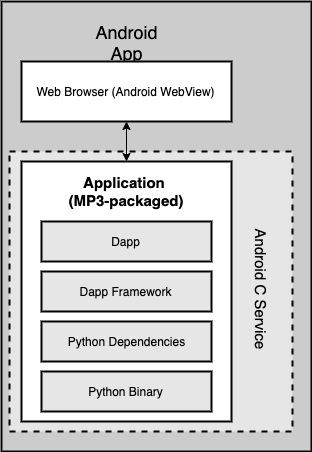
\includegraphics[width=0.5\textwidth]{images/android-app.png}
	\caption{\label{fig:android-architecture}}
\end{figure}

Since the Android app is needed to interact with the C service in the background, a part of the app had to be written in either Java or Kotlin. To keep this amount of code to a minimum, a decision was made to create all GUIs in web technologies, so the view layer can be shared between mobile and desktop platforms. This decision made it possibly to include a web browser as the only component written for the mobile platform. This web browser can then interact with the web server and REST API running on the C service.

To package the executable code in a way that would not trigger the Android security system, the code had to be bundled in a single file, disguised as a MP3. This format does not get checked by the Android security system  and therefore can be used for the purpose of this work. Underneath the extenstion, the code is packaged as a GZIP Tar-archive. Upon running the Android application, this MP3 file is unpacked in the application space of the app and the C service is started with the right configuration to run the code.

In Figure~\ref{fig:android-app} a screenshot can be seen of the framework running with a test dApp on the Android platform. Development was stopped after reaching the proof-of-concept stage as it is not the main goal of this work and the development cycle is very tedious and slow. Each time a change or addition is made to the Framework the entire app structure has to be rebuild. This process can take up to 20 minutes. 

\begin{figure}[h!]
	\centering
	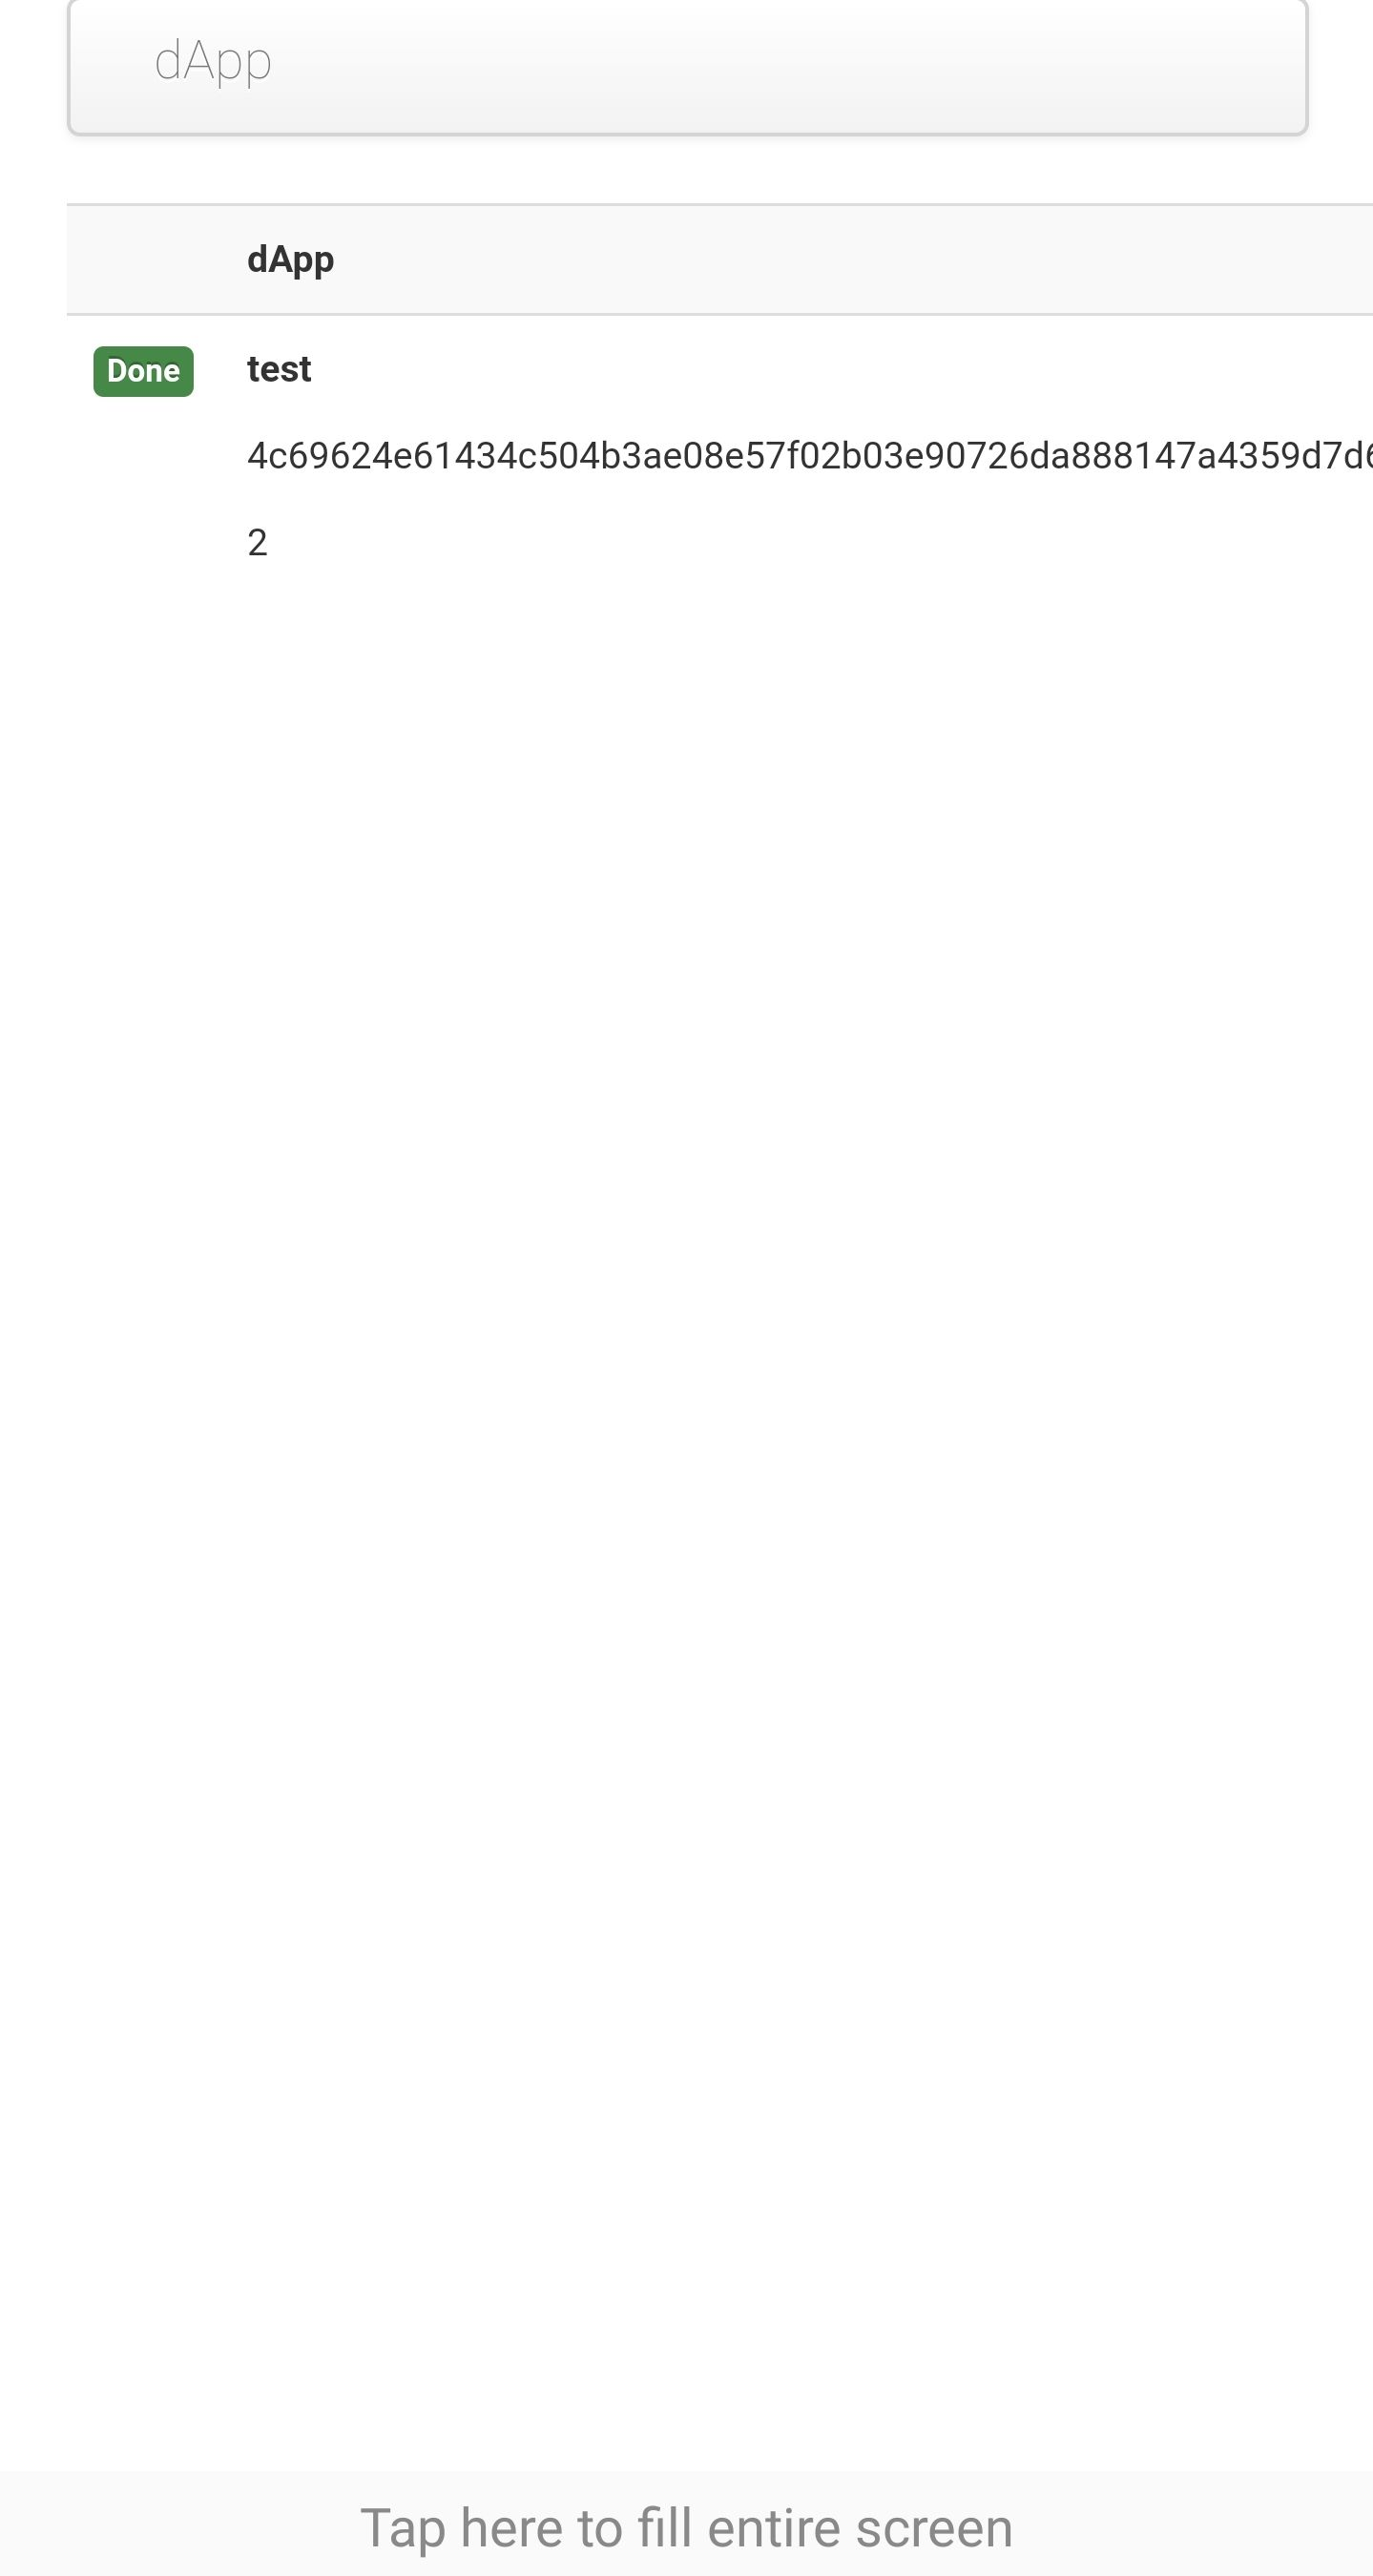
\includegraphics[width=0.5\textwidth]{images/android-app-screenshot.jpg}
	\caption{\label{fig:android-app}}
\end{figure}
